% document class
\documentclass[11pt, a4paper, onecolumn, fleqn, twoside, titlepage, openright]{book}

% packages
\usepackage[twoside, top=1.6in, bottom=0.9in, left=1.25in, right=1in, 
			bindingoffset=0.25in, heightrounded]{geometry}
\usepackage[round, authoryear]{natbib} 
\usepackage[bitstream-charter]{mathdesign}
\usepackage[sc]{mathpazo}
\usepackage{tocbibind}
\usepackage{graphicx}
\usepackage{sidecap}
\usepackage{fancyhdr}
\usepackage[grey, charter]{quotchap}
\usepackage[colorlinks=true,
 			a4paper=true,
 			linktocpage=true,
 			pagebackref=true,
 			pageanchor=true,
 			hyperindex=true,
 			bookmarks=true,
 			bookmarksopen=true,
 			bookmarksnumbered=true,
 			pdffitwindow=true,
 			citecolor=blue,
 			urlcolor=blue]{hyperref}



\begin{document}

	%%%%%%%%%%%%%%%%%%%%%%%%%%%%%%%%%% TITLE PAGE %%%%%%%%%%%%%%%%%%%%%%%%%%%%%%%%%%
	\thispagestyle{empty}

	\begin{center}
	    \begin{minipage}{0.75\linewidth}
	        \centering
	        %University logo
	        
\includegraphics[width=0.5\linewidth]{images/logo_unipd.pdf}
	        \vspace{3cm}
	    
	        %Thesis title
	        {\Large \textbf{The title of my thesis project} \par}
	        \vspace{3cm}
	    
	        %Author's name
	        \hspace{5cm}
	        \textbf{Candidate:} Nicola Dal Lago
	        \vspace{3cm}

	        %Supervisors' names
	        \hspace{-8.7cm}\textbf{Advisor:} Prof. Luca Schenato \\
	        \hspace{-7.1cm}\textbf{Advisor:} Prof. George Nikolakopoulos \\
	        \hspace{-11.8cm}\textbf{Advisor:} ...
	        \vspace{3cm}

	        %Degree
	        Master in Control Engineering \\
	        Department of Information Engineering \\ 
	        2016
	        
	    \end{minipage}
	\end{center}

	\clearpage
	%%%%%%%%%%%%%%%%%%%%%%%%%%%%%%%%%% TITLE PAGE %%%%%%%%%%%%%%%%%%%%%%%%%%%%%%%%%%


	%%%%%%%%%%%%%%%%%%%%%%%%%%%%%%%%%%% ABSTRACT %%%%%%%%%%%%%%%%%%%%%%%%%%%%%%%%%%%
	\chapter*{Abstract}
	\label{abstract}

	\begin{quote}
		This is my abstract
	\end{quote}
	%%%%%%%%%%%%%%%%%%%%%%%%%%%%%%%%%%% ABSTRACT %%%%%%%%%%%%%%%%%%%%%%%%%%%%%%%%%%%


	\tableofcontents	


	%%%%%%%%%%%%%%%%%%%%%%%%%%%%%%%%% INTRODUCTION %%%%%%%%%%%%%%%%%%%%%%%%%%%%%%%%%
	\chapter{Introduction}
	\label{introduction}

	In these last years, a growing interest has been shown in robotics, In fact, several industries (automotive, medical, manufacturing, space, etc.), require robots to replace men in dangerous, repetitive or onerous situations. A wide area of this research is dedicated to Unmaned Aerial Vehicle (UAV) and especially the one of having the capability of Vertical TakeOff and Landing (VTOL) \cite{modelIdentification}. This kind of vehicle can be use in a variety of different scenario, do to the reasonable price, small dimensions and large sensors capability. In particular, nowdays intensive research as been accomplish in the area of enviroment monitoring and exploration, accomplish with different strategies and sensors.

	\begin{SCfigure}[\sidecaptionrelwidth][h!]
		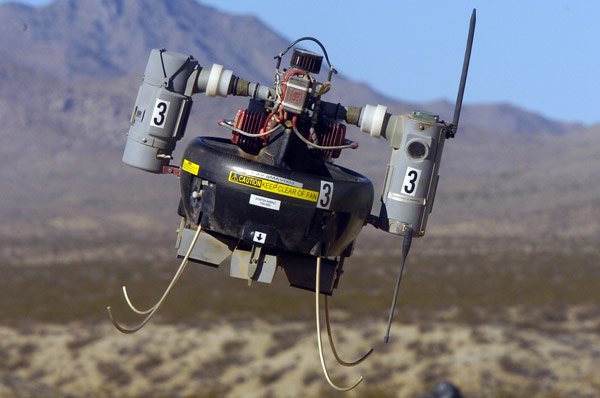
\includegraphics[scale=0.4]{images/fukushima.jpg}
		\caption{T-Hawk, a US-made UAV, commonly used to search for roadside bombs in Iraq, made its debut when it photographed the Fukushima nuclear plant from above, providing a detailed look at the interior damage.}
		\label{fig:application}
	\end{SCfigure}  

	\noindent Many typse of UAVs have been developed over the last years, in particular the quadrotor type \cite{LeeController}, a quadrotor type UAV consists of two pairs of counter rotating rotors and propellers. The aim of this thesis is to contribute to the develop of the so called \textit{Prometheus project}, a fully autonomus vertical tekeoff and landing vehicle, able to perform indoor enviroment exploration and mapping. To do this, we inspired from the film Prometheus, where drones are able to map an indoor cave. Of course, do to technology and budjet limitations, the vehicle will not have the same performance, but will have in theory the same capabilities. As previously said, this thesis is only a part of the project, that has been diveded in three main parts:

	\begin{itemize}
		\item mechanical design and building of the UAV;
		\item mathematical model, system identification and control;
		\item usage of the sensors, mapping and navigation alghoritms.
	\end{itemize}

	\noindent This thesis will focus on the second point, but brefly introductions will give also in the other two points, in particular in the mechanical design, necessary for develop a mathematical model. 

	\begin{SCfigure}[\sidecaptionrelwidth][h!]
		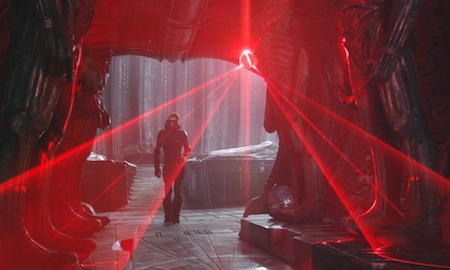
\includegraphics[scale=0.6]{images/prometheus_film.jpg}
		\caption{Frame of the prometheus movie, where the drone perform the exploration and mapping of the cave.}
		\label{fig:prometheusFILM}
	\end{SCfigure}

	\noindent Description of the varius chapters........
	%%%%%%%%%%%%%%%%%%%%%%%%%%%%%%%%% INTRODUCTION %%%%%%%%%%%%%%%%%%%%%%%%%%%%%%%%%










	%%%%%%%%%%%%%%%%%%%%%%%%%%%%%%% DESIGN AND MODEL %%%%%%%%%%%%%%%%%%%%%%%%%%%%%%%
	\chapter{Design and model}
	\label{designModel}

	In this chapter we will focus in the description of the mechanical model of the UAV and the sensor system and, from these, a mathematical model will derive, necessary for build and simulate a control law, and to perform system identification.

	\section{Mechanical design}
	\label{mechanicalDesign}


	%%%%%%%%%%%%%%%%%%%%%%%%%%%%%%% DESIGN AND MODEL %%%%%%%%%%%%%%%%%%%%%%%%%%%%%%%











	%%%%%%%%%%%%%%%%%%%%%%%%%%%%%%%%% BIBLIOGRAPHY %%%%%%%%%%%%%%%%%%%%%%%%%%%%%%%%%
	\begin{thebibliography}{1}
	\label{bibliography}

		\bibitem{modelIdentification}
		\textbf{Emil Fresk, R. James Cotton and George Nikolakopoulos}
		Generalized Model Identification for Multirotors: Towards applications in Auto Tunning.
		\textit{2016}.

		\bibitem{LeeController}
		\textbf{Taeyoung Lee, Melvin Leok and N. Harris McClamroch}
		Nonlinear Robust Tracking Control of a Quadrotor UAV on $SE(3)$.
		\textit{2012 American Control Conference, Fairmont Queen Elizabeth, Montréal, Canada, June 27 - June 29, 2012}.

	\end{thebibliography}
	%%%%%%%%%%%%%%%%%%%%%%%%%%%%%%%%% BIBLIOGRAPHY %%%%%%%%%%%%%%%%%%%%%%%%%%%%%%%%%

\end{document}
